\documentclass[final]{beamer}
\usepackage{multimedia}
\usepackage{color}
\usepackage[normalem]{ulem}
\graphicspath{{figures/}}

\newcommand{\comment}[1]{}
\definecolor{grigio}{rgb}{.8, .8, .8}

\mode<beamer>{%
	\usetheme{default}
  \usecolortheme{default}
}
\titlegraphic{
\includegraphics[width=0.3\textwidth]{LogoUPF_CBC}\hspace{0.5cm}
\includegraphics[width=0.3\textwidth]{logo_italian_academy}\hspace{0.5cm}
\includegraphics[width=0.15\textwidth]{columbia}}
\title[Effective connectivity]{\textbf{Whole brain effective connectivity from fMRI data}\\ Some subtitle}
\author{Andrea Insabato}
\date{November 27th, 2017}

\begin{document}


\begin{frame}<handout:0>
  \titlepage
\end{frame}

\begin{frame}
\transdissolve
\frametitle{Whole brain connectivity}
\begin{columns}
\begin{column}{0.5\textwidth}
	\begin{itemize}
			\pause
		\item Whole brain is divided in ROIs (parcellation)
			\pause
		\item Average activity in each ROI
			\pause
		\item Connectivity between ROIs
	\end{itemize}
\end{column}
\begin{column}{0.5\textwidth}
\includegraphics<1->[width=0.5\columnwidth,valign=t]{brain_connectivity}
\end{column}
\end{columns}
\end{frame}

\begin{frame}
\transdissolve
\frametitle{Functional Connectivity (FC)}
\begin{columns}
\begin{column}{0.5\textwidth}
\includegraphics<1->[width=0.5\columnwidth,valign=t]{FC}
\end{column}
\begin{column}{0.5\textwidth}
	\begin{itemize}
			\pause
		\item Pearson correlation between ROIs
			\pause
		\item Dense 
			\pause
		\item Symmetric: no directionality of interactions 
	\end{itemize}
\end{column}
\end{columns}
\end{frame}

\begin{frame}
\transdissolve
\frametitle{Effective Connectivity (EC)}
\begin{columns}
\begin{column}{0.5\textwidth}
\includegraphics<1->[width=0.5\columnwidth,valign=t]{EC}
\end{column}
\begin{column}{0.5\textwidth}
	\begin{itemize}
			\pause
		\item Network model 
			\pause
		\item Sparse 
			\pause
		\item Asymmetric: no directionality of interactions 
	\end{itemize}
\end{column}
\end{columns}
\end{frame}

\begin{frame}
\transdissolve
\frametitle{Outline}
\begin{itemize}
		\pause
	\item Network model
		\pause
	\item EC based subject and condition identification
		\pause
	\item Estimation of model parameters
\end{itemize}
\end{frame}

\begin{frame}
\transdissolve
\frametitle{Network model}
\begin{itemize}
		\pause
	\item Each node is an Ornstein-Uhlenbeck process 
		\pause
	\item $dx_i(t) = [-\frac{x_i(t)}{\tau_i} + \sum_{j\ne i} C_{ij} x_j + \eta_i]dt + dB_i;\qquad dB_i\sim\mathcal{N}(0,\sigma_i^2)$ 
		\pause
\end{itemize}
\end{frame}

\begin{frame}
\frametitle<1>{Characterization of whole brain networks underlying ``mental'' states}
\frametitle<2>{Characterization of whole brain networks underlying watching a movie}
\frametitle<3>{Characterization of whole brain networks underlying remembering}
\frametitle<4>{Characterization of whole brain networks underlying calculating}
\frametitle<5>{Characterization of whole brain networks underlying pathological states (dementia, autism, depression, etc.)}
\frametitle<6->{Characterization of whole brain networks underlying ``mental'' states}
\transdissolve
\begin{itemize}
	\item<7-> Separate different sources of varibility
\end{itemize}
\begin{center}
	\visible<8->{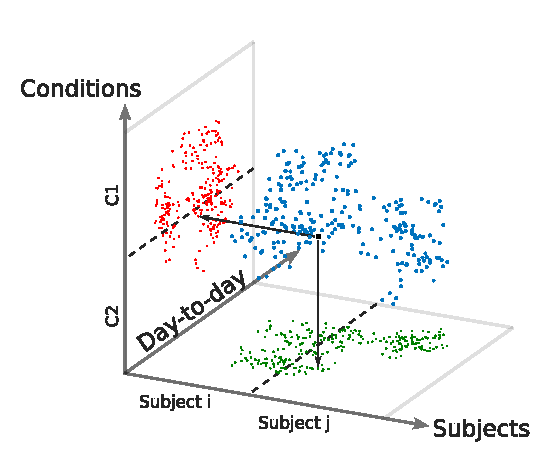
\includegraphics[width=0.5\columnwidth,valign=b]{subj_cond_idea}}
\end{center}
\end{frame}

\begin{frame}
\transdissolve
\frametitle{Characterization of whole brain networks underlying ``mental'' states}
\begin{itemize}
\pause
	\item watching a movie, remembering, calculating, pathological states (dementia, autism, depression, etc.) 
\pause
	\item Separate different sources of varibility
\pause
	\begin{itemize}
		\item classify individuals
			\pause
		\item classify conditions 
			\pause
		\item extract networks underlying each classification
	\end{itemize}
\end{itemize}
\end{frame}


\begin{frame}
\frametitle{Acknowledgments}
\begin{columns}
\begin{column}{0.5\textwidth}
\begin{center}
	\alert<2>{Vicente Pallares}\\
\vspace{1cm}

\alert<2>{Matthieu Gilson}\\
\vspace{1cm}

\small Ana Sanjuan\\
\vspace{0.5cm}

\small Simone Kuhn\\
\vspace{0.5cm}

\small Dante Mantini\\
\vspace{0.5cm}

\small Gustavo Deco\\
\end{center}
\end{column}
\begin{column}{0.5\textwidth}
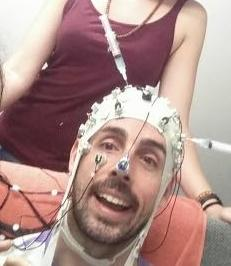
\includegraphics[width=0.5\columnwidth,valign=t]{vicente2}
\vspace{0.5cm}

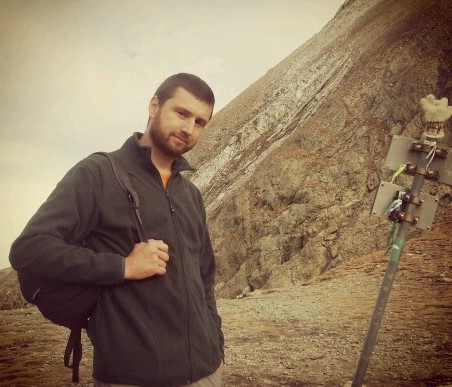
\includegraphics[width=0.5\columnwidth,valign=t]{matt}
\end{column}
\end{columns}
\end{frame}


\end{document}
